\chapter{Fundamentals of Retrieval-Augmented Generation}
\label{chap:fundamentals_rag}

Retrieval-Augmented Generation (RAG) systems represent a paradigm shift in how Large Language Models interact with information, combining the generative capabilities of pre-trained models with the precision of information retrieval systems \autocite{rag_survey_2024_ralm}. This chapter lays the groundwork by explaining the core mechanics of RAG, the primary challenges in its implementation, the critical role of vector databases, and the strategies for mitigating common failure points like LLM hallucinations.

\section{How it Works}
At its core, a RAG system operates in two main stages: retrieval and generation. The process begins when a user submits a query. Instead of directly feeding the query to the LLM, the RAG pipeline intercepts it and first interacts with an external knowledge base.

\begin{enumerate}
    \item \textbf{Retrieval Stage:} The user's query is converted into a numerical representation, or \textit{embedding}, using a text embedding model. This query embedding is then used to search a pre-indexed collection of documents. The goal is to find and retrieve chunks of text that are semantically similar to the query. This retrieval is typically performed using a vector database, which is optimized for high-speed similarity searches over large datasets of embeddings. The output of this stage is a set of relevant text chunks, often referred to as the \textit{context}.
    
    \item \textbf{Generation Stage:} The retrieved context is then combined with the original query into a structured prompt. This augmented prompt is fed to the LLM. By providing this explicit, relevant information, the LLM is guided to generate a response that is not only contextually appropriate but also grounded in the facts contained within the retrieved documents. This process significantly enhances the accuracy and factuality of the output.
\end{enumerate}

\begin{figure}[!htbp]
    \centering
    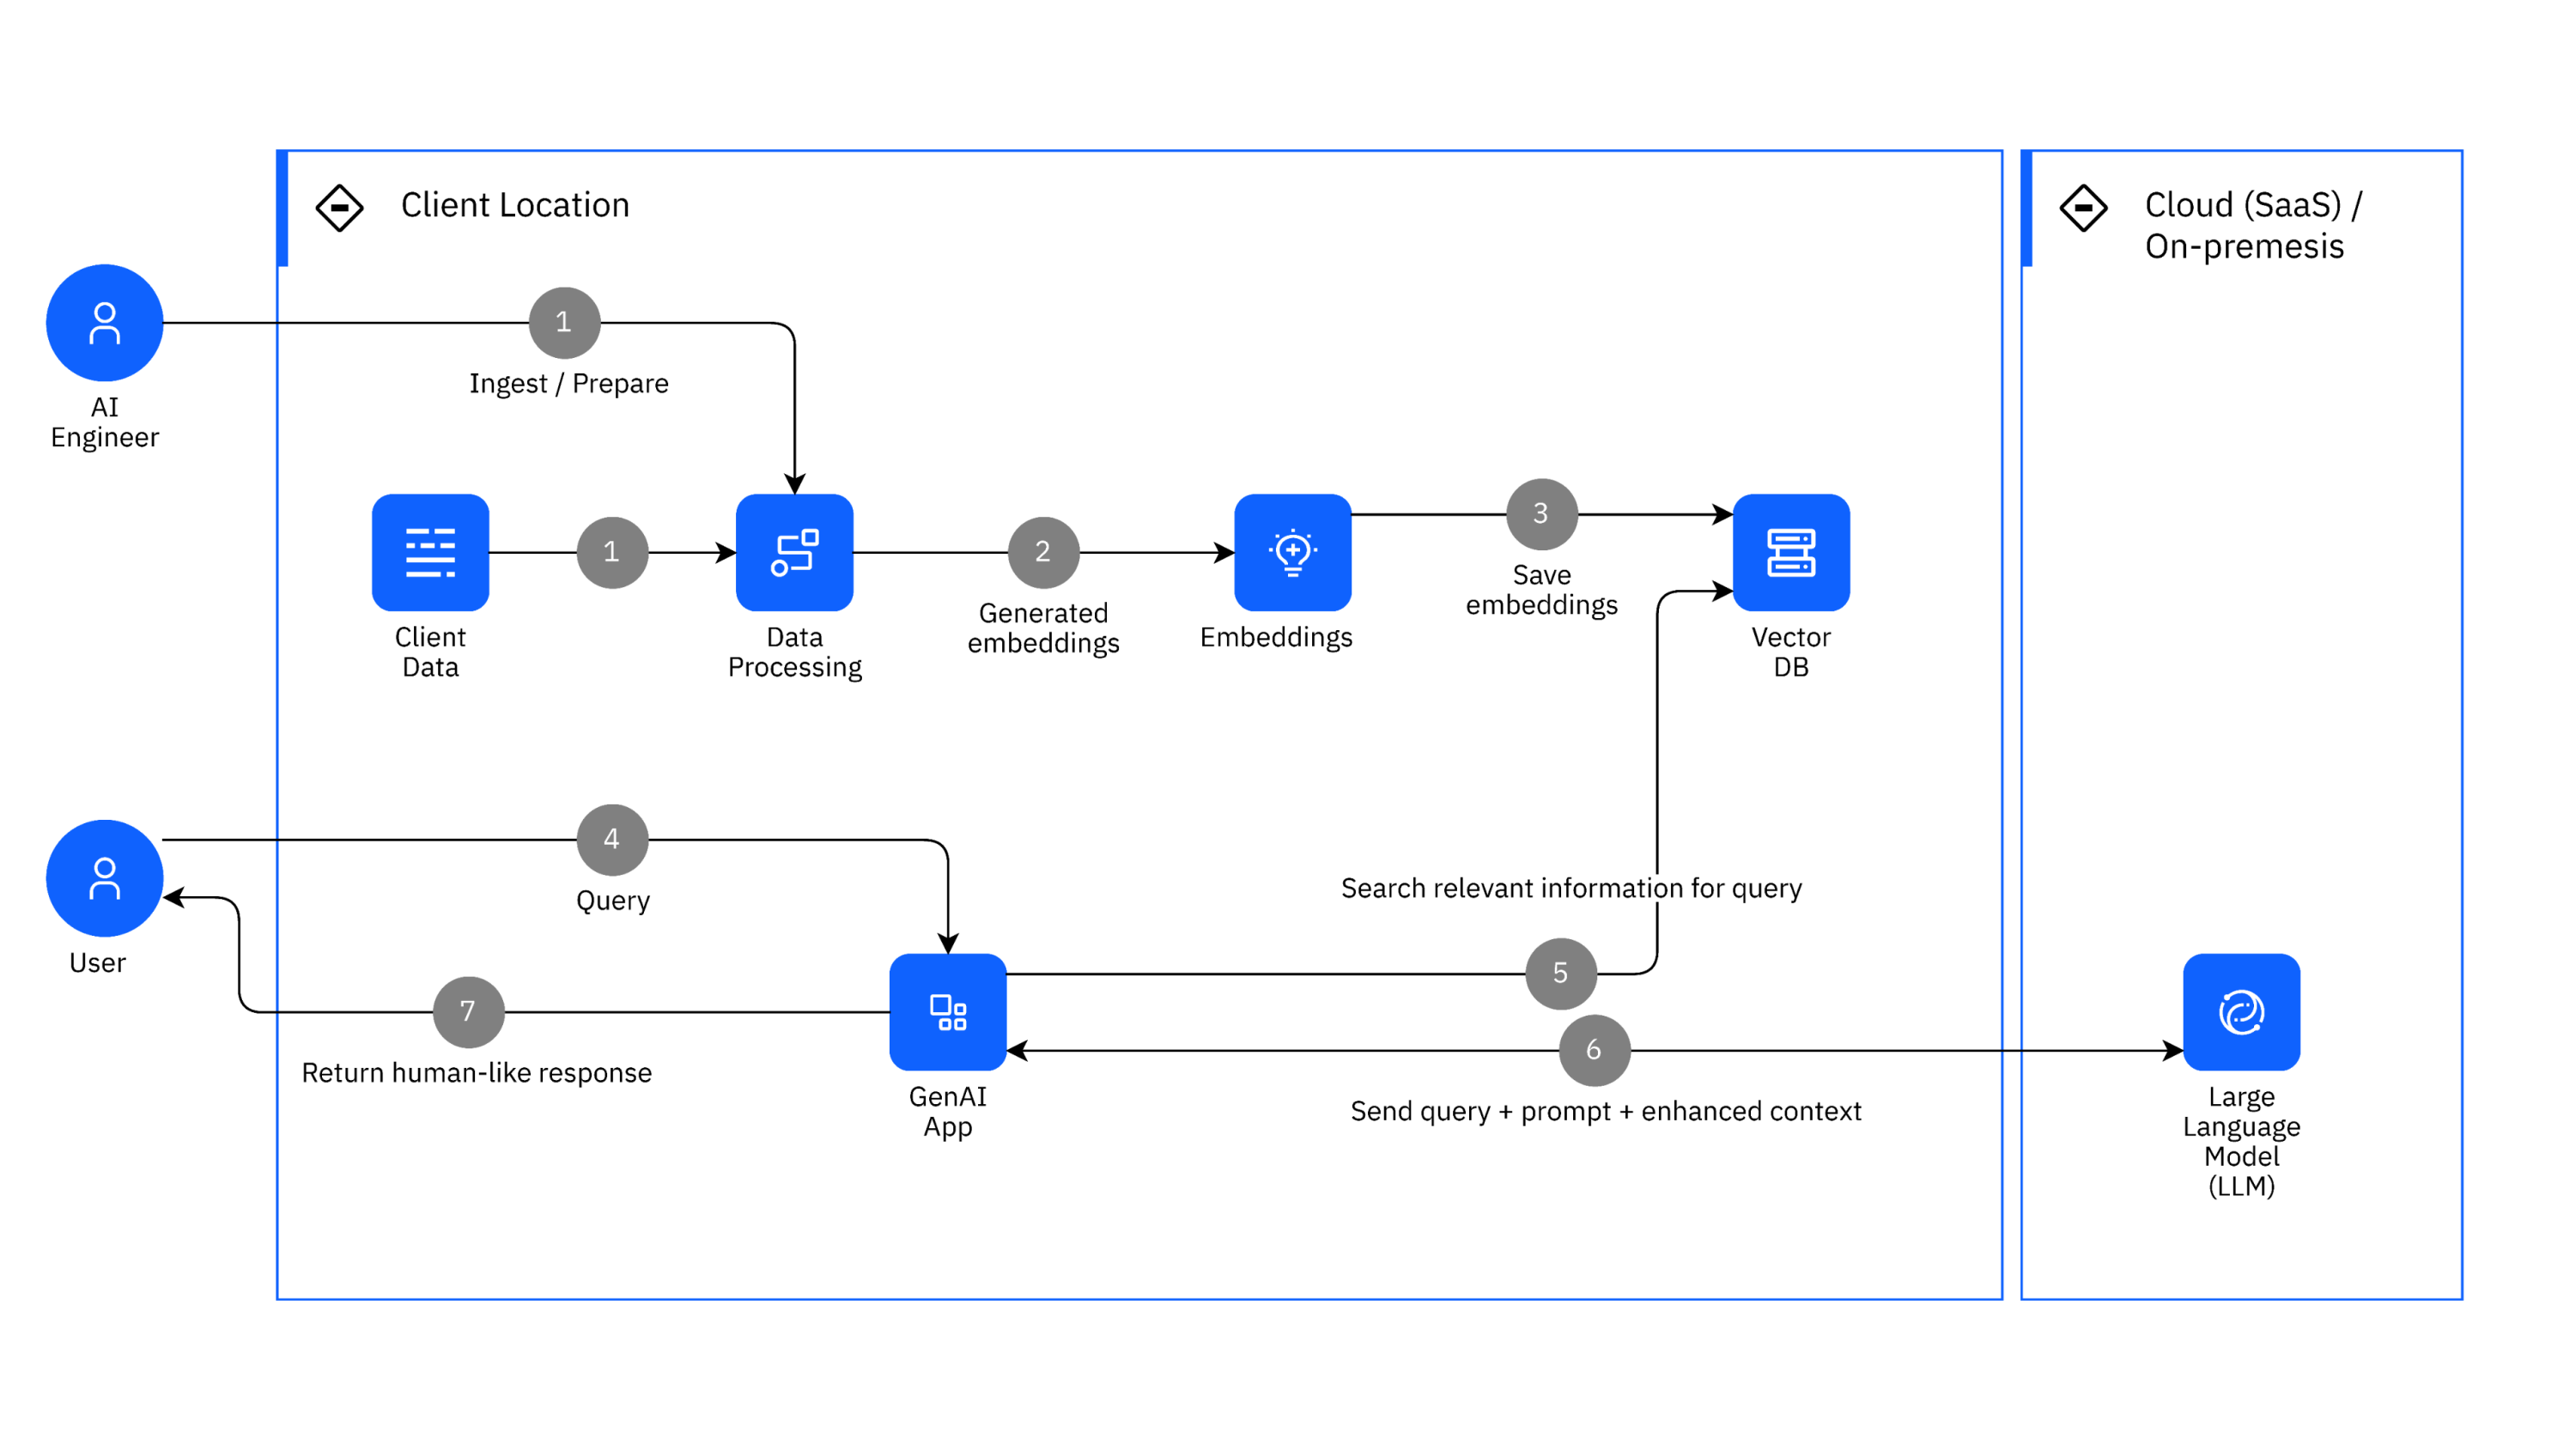
\includegraphics[width=0.9\textwidth]{images/chapter2/rag_architecture.png}
    \caption{High-level architecture of a Retrieval-Augmented Generation system. Image from IBM \autocite{ibm-rag-pattern}.}
    \label{fig:rag_architecture}
\end{figure}

\section{Main Challenges}
The apparent simplicity of the RAG pipeline belies several complex challenges that must be addressed to build a robust and effective system:
\begin{itemize}
    \item \textbf{Ensuring Content Relevance:} The quality of the generated output is fundamentally dependent on the quality of the retrieved context. If the retriever fetches irrelevant or low-quality documents, the LLM may ignore them or, worse, incorporate incorrect information into its response. A key challenge is the \textit{lost in the middle problem}, where LLMs tend to overlook relevant information if it is buried among less relevant chunks in the context window.
    \item \textbf{Optimizing Retrieval vs. Generation Trade-offs:} There is an inherent trade-off between the speed and comprehensiveness of the retrieval step. Retrieving more documents might increase the chance of finding the correct information but also increases the computational load and the risk of introducing noise. The length of the context that can be passed to the LLM is also limited by its context window size.
    \item \textbf{Handling Noisy or Conflicting Information:} Real-world data is often messy. The retrieved context may contain conflicting facts or irrelevant details. The RAG system must be resilient to such noise, and the LLM must be capable of synthesizing information from multiple sources, identifying contradictions, and prioritizing the most reliable data.
    \item \textbf{Seamless Integration and Synthesis:} The LLM must be able to seamlessly weave the retrieved information into a coherent and natural-sounding response. This requires not just extracting facts but understanding the nuances of the context and integrating them into a cohesive narrative that directly answers the user's query.
\end{itemize}

\section{Vector Databases and Similarity Search}Vector databases are a cornerstone of modern RAG systems. They work by storing text data as high-dimensional vectors known as \textit{embeddings}. When a query is received, it is also converted into an embedding, and the database searches for the vectors in its index that are closest to the query vector.\subsection{Measuring Similarity}The most common way to measure the distance between two vectors in the context of RAG is \textbf{cosine similarity}, which measures the cosine of the angle between them. For two vectors, A and B, the cosine similarity is calculated as:\begin{equation}\text{Cosine Similarity} = \frac{A \cdot B}{\|A\| \|B\|}\end{equation}Where \(A \cdot B\) is the dot product of the two vectors, and \(\|A\|\) and \(\|B\|\) are their magnitudes. The result ranges from -1 (exactly opposite) to 1 (exactly the same).Another common metric is \textbf{Euclidean distance}, which is the straight-line distance between two points in the vector space:\begin{equation}\text{Euclidean Distance} = \sqrt{\sum_{i=1}^{n} (A_i - B_i)^2}\end{equation}\subsection{The Advantage of Normalized Vectors}For efficiency, it is a common practice to \textbf{normalize} the vectors before storing them in the database. A normalized vector has a magnitude (or L2 norm) of 1. When vectors are normalized, the denominator in the cosine similarity formula (\(\|A\| \|B\|\)) becomes 1. Therefore, the cosine similarity calculation simplifies to just the \textbf{dot product} of the vectors:\begin{equation}\text{Cosine Similarity (normalized)} = A \cdot B\end{equation}This is computationally much cheaper, as it avoids the expensive square root operations needed to calculate the vector magnitudes. This optimization allows for significantly faster similarity searches, which is critical for real-time RAG applications.\subsection{Indexing for Efficient Search}To avoid a brute-force search, vector databases use specialized indexing algorithms for Approximate Nearest Neighbor (ANN) search. Two of the most prominent are:\begin{itemize}    \item \textbf{Hierarchical Navigable Small World (HNSW):} This is a graph-based approach where vectors are represented as nodes in a multi-layered graph. The search starts at a random entry point in the top layer (which has the fewest nodes) and navigates towards the target. It then moves to a lower, more densely populated layer to refine the search, quickly converging on the nearest neighbors \autocite{hnsw_malkov_2018}.    \item \textbf{Inverted File (IVF):} This method first clusters the vectors into a set of partitions. When a query comes in, it is first compared to the cluster centroids to find the most promising partitions. The search is then performed only on the vectors within those selected partitions, significantly reducing the search space \autocite{ivf_jegou_2011}.\end{itemize}These ANN algorithms provide a highly efficient way to find semantically similar results without having to compare the query to every single item in the database, making large-scale RAG feasible.

\section{Mitigating Hallucinations}
One of the most significant benefits of RAG is its ability to mitigate LLM hallucinations. By providing factual, verifiable context directly within the prompt, RAG grounds the model's response in reality. The LLM is instructed to formulate its answer based on the provided text, reducing its reliance on its internal, parametric knowledge, which may be outdated or incorrect.

However, RAG is not a perfect solution. If the retrieved context is of poor quality, contains subtle inaccuracies, or is itself misleading, the LLM may still generate a flawed response. Therefore, the quality of the retrieval process is paramount. A well-tuned retriever that provides accurate and relevant context is the first and most critical line of defense against hallucinations in a RAG system \autocite{rag_prompt_eng_guide}.